Recurrent neural networks differ from feed foward neural networks because of the presence of recurrent connections: at least one perceptron output at a given layer $i$ is \textit{fed} to another perceptron
at a level $j<i$, as can be seen in figure \ref{rnn_model}. This is a key difference: as we will see in the next section, rnn are not only more powerfull than ffnn but as powerfull as turing machines.


\tikzstyle{rnn_style}=[->,shorten >=1pt,auto,node distance=1.5cm,
  thick,
  neuron/.style={circle,fill=white!50,draw,minimum size=0.7cm,font=\sffamily\Large\bfseries},
  missing/.style={circle,fill=white!50,draw=none,minimum size=0.7cm,font=\sffamily\Huge\bfseries},
  label/.style={node distance=1.2cm,rectangle,fill=white!50,draw=none,minimum size=0.7cm,font=\sffamily\normalsize},
  layer/.style={rectangle,fill=white!50,draw,minimum width=4cm,font=\sffamily\normalsize},
  loopStyle/.style={in=120,out=60, distance=2.5cm},]
\begin{figure}[h!]
 \centering
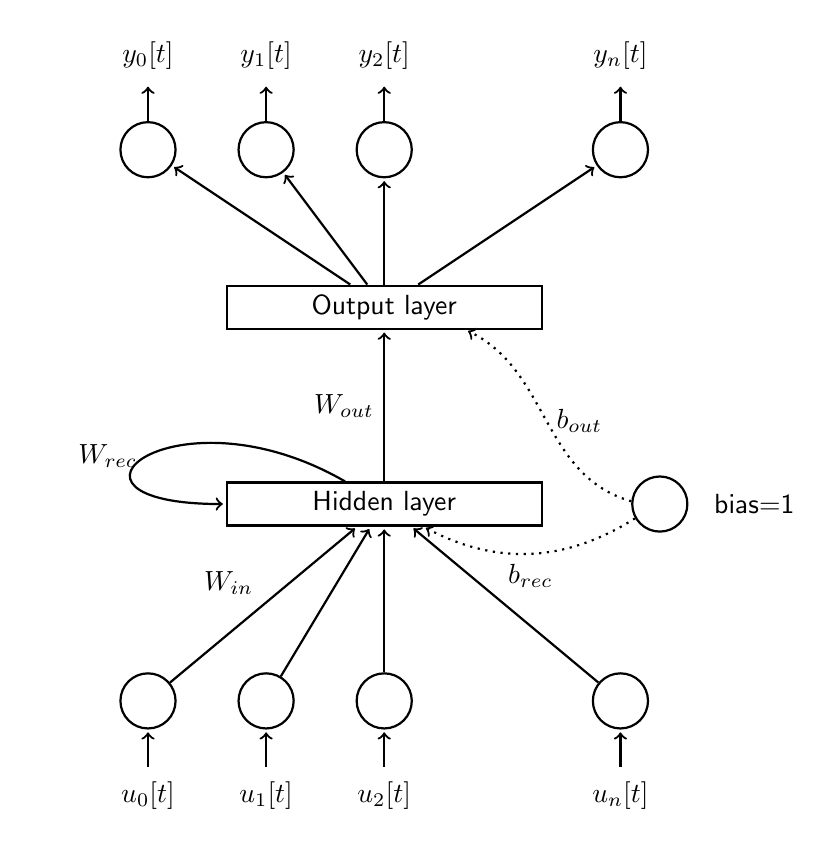
\begin{tikzpicture}[rnn_style]

  \node[neuron]    (x0)       {};
  \node[neuron]    (x1)[right of=x0]   {};
  \node[neuron]    (x2)[right of=x1]   {};
  \node[missing]   (x3)[right of=x2]   { $\hdots$};
  \node[neuron]    (xn)[right of=x3]   {};
  
  \node[label]    (u0)[below of=x0]   {$u_0[t]$};
  \node[label]    (u1)[below of=x1]   {$u_1[t]$};
  \node[label]    (u2)[below of=x2]   {$u_2[t]$};
  \node[label]    (un)[below of=xn]   {$u_n[t]$};
  
  
  
  \node[layer] (hl)[above of=x2,node distance=2.5cm] {Hidden layer};
  \node[neuron](b) [right of=hl,node distance=3.5cm] {};
  \node[label] (b_l) [right of=b] {bias=1};
  \node[layer] (ol)[above of=hl,node distance=2.5cm] {Output layer};
  
  \node[neuron] (o1) at (0,7) {};
  \node[neuron] (o2)[right of=o1] {};
  \node[neuron] (o3)[right of=o2] {};
  \node[missing](o4)[right of=o3] {$\hdots$};
  \node[neuron] (on)[right of=o4] {};
  
  
  \node[label]    (y0)[above of=o1]   {$y_0[t]$};
  \node[label]    (y1)[above of=o2]   {$y_1[t]$};
  \node[label]    (y2)[above of=o3]   {$y_2[t]$};
  \node[label]    (yn)[above of=on]   {$y_n[t]$};
  
  
  \path[->] (x0) edge [] node[]{$W_{in}$}   (hl)
	    (x1) edge []   (hl)
	    (x2) edge []   (hl)
	    (xn) edge []   (hl)
	    (u0) edge []   (x0)
	    (u1) edge []   (x1)
	    (u2) edge []   (x2)
	    (un) edge []   (xn)
	    (ol) edge []   (o1)
	    (ol) edge []   (o2)
	    (ol) edge []   (o3)
	    (ol) edge []   (on)
	    (o1) edge []   (y0)
	    (o2) edge []   (y1)
	    (o3) edge []   (y2)
	    (on) edge []   (yn)
	    (hl) edge []  node[]{$W_{out}$} (ol)
	    (b)  edge [bend left,dotted]  node[]{$b_{rec}$} (hl)
	    (b)  edge [bend left,dotted,anchor=west, in= -160]  node[]{$b_{out}$} (ol)
	    (hl) edge [loop ,in=-180,out=150, distance=2.5cm,anchor=east ]      node [align=center]  {$W_{rec} $} (hl);


\end{tikzpicture}
\caption{Rnn model}
\label{rnn_model}
\end{figure}



This difference in topology reflects also on the network's input and output domain, where in feed foward neural networks inputs and outputs were real valued vectors, recursive neural networks deal with
sequences of vectors, that is to say that now time is also considered. One may argue that taking time (and sequences) into consideration is some sort of limitation because it restricts our model to deal only
with a temporal inputs; that's not true, in fact we can apply rnn to non temporal data by considering space as the temporal dimension or we can feed the network with the same input for all time steps, or just
providing no input after the first time step.

\begin{defn}[Recurrent neural network]
\label{def_rnn}
A recurrent  neural network is tuple
$$RNN\triangleq< W_{in}, W_{out}, W_{rec},\vec{b}_{out}, \vec{b}_{rec} ,\sigma(\cdot),f(\cdot)>$$
\begin{itemize}
 \item $W^{in}$ is the $r\times p$ input weight matrix
 \item $W^{rec}$ is the $r\times r$ recurrent weight matrix
 \item $W^{out}$ is the $o \times r$ output weight matrix
 \item $\vec{b}^{rec} \in \mathbb{R}^{r}$ is the bias vector for the recurrent layer
 \item $\vec{b}^{out} \in \mathbb{R}^{o}$ is the bias vector for the output layer
 \item $\sigma(\cdot): \mathbb{R}\rightarrow \mathbb{R}$ is the activation function
 \item $F(\cdot): \mathbb{R}^{o)}\rightarrow \mathbb{R}^{o}$ is the output function
\end{itemize}
$p$ is the size of input vectors, $r$ is the number of hidden units, $o$ is the size of output vectors. 
The total number of weights si given by $\mathcal{N}(W) \triangleq rp+r^2+ro$, the number of biases by $\mathcal{N}(b) \triangleq r+o $
\end{defn}

Given a $RNN$ and an input sequences $\{\vec{x}\}_t$ the output sequence $\{\vec{y}\}_t$ of the net is defined by the following:
\begin{align}
&\vec{y}_t \triangleq f(W^{out}\cdot\vec{\phi}_t + \vec{b}^{out})\\
&\vec{a}_t \triangleq W^{rec}\cdot\vec{\phi}_{t-1}+W^{in}\cdot\vec{x}_t+\vec{b}^{rec}\\
&\vec{\phi}_t \triangleq  \sigma(\vec{a}_t)
\end{align}

As we can understand from definition \ref{def_rnn}, there is only one recurrent layer, whose weights are the same for each time step, so one can asks where does the deepness of the network come from.
The answer lies in the temporal unfolding of the network, in fact if we unfold the network step by step we obtain a structure similar to the structure of a feed foward neural network. As we can observe
in figure \ref{rnn_unfolding}, the unfolding of the network through time consist of putting identical version of the same reccurent layer on top of each other and linking the inputs of one layer to the
next one. The key difference from feed foward neural networks if, as we have already observed, that the weights in each layer are identical, and of course the additional timed inputs which are different for
each unfolded layer.

\tikzstyle{rnn_style}=[->,shorten >=1pt,auto,node distance=1.5cm,
  thick,
  neuron/.style={circle,fill=white!50,draw,minimum size=0.7cm,font=\sffamily\Large\bfseries},
  missing/.style={circle,fill=white!50,draw=none,minimum size=0.7cm,font=\sffamily\Huge\bfseries},
  label/.style={node distance=1.2cm,rectangle,fill=white!50,draw=none,minimum size=0.7cm,font=\sffamily\normalsize},
  layer/.style={rectangle,fill=white!50,draw,minimum width=4cm,font=\sffamily\normalsize},
  loopStyle/.style={in=120,out=60, distance=2.5cm},]
\begin{figure}[h!]
 \centering
\begin{tikzpicture}[rnn_style]

  %t=0
  \node[layer] (hl1) {Hidden layer t=0};
  
  \node[neuron]    (x0)[below left=0.3cm and 1cm of hl1]       {};
  \node[label]    (u0)[left of=x0]   {$\vec{x}_1$};
  

  
  \node[neuron] (o0) [above right=0.3cm and 1cm of hl1] {};
  \node[label]    (y0)[right of=o0]   {$\vec{y}_1$};
  
  %t=1
  \node[layer] (hl2)[above of=hl1,node distance=2.5cm] {Hidden layer t=1};
  
  \node[neuron]    (x1)[below left=0.3cm and 1cm of hl2]      {};
  \node[label]    (u1)[left of=x1]   {$\vec{x}_2$};
  
    
  \node[neuron] (o1) [above right=0.3cm and 1cm of hl2] {};
  \node[label]    (y1)[right of=o1]   {$\vec{y}_2$};
  
  %dots
  \node[label,font=\sffamily\Huge\bfseries] (hld)[above of=hl2,node distance=2cm] {$\hdots$};
  
  %t=T
  \node[layer] (hlT)[above of=hld,node distance=2cm] {Hidden layer t=T};
  
  \node[neuron]    (xT)[below left=0.3cm and 1cm of hlT]      {};
  \node[label]    (uT)[left of=xT]   {$\vec{x}_T$};
  
    
  \node[neuron] (oT) [above right=0.3cm and 1cm of  hlT] {};
  \node[label]    (yT)[right of=oT]   {$\vec{y}_T$};
  
  
  %biases
  \node[neuron](b) [right of=y1,node distance=2cm] {};
  \node[label] (b_l) [right of=b] {bias=1};

  
  \path[->] (x0) edge [bend right] node[]{$W^{in}$}   (hl1)
	    (u0) edge []   (x0)
	    (o0) edge []   (y0)
	    (x1) edge [bend right] node[]{$W^{in}$} (hl2)
	    (u1) edge []   (x1)
    	    (o1) edge []   (y1)
	    (xT) edge [bend right] node[]{$W^{in}$} (hlT)
	    (uT) edge []   (xT)
    	    (oT) edge []   (yT)

	    
	    (hl1) edge [bend left]  node[]{$W^{out}$} (o0)
    	    (hl2) edge [bend left]  node[]{$W^{out}$} (o1)
    	    (hlT) edge [bend left]  node[]{$W^{out}$} (oT)

	    (b)  edge [bend left,dotted,in = 90]  node[]{$b^{out}$} (o0)
	    (b)  edge [bend left, dotted, in = 90,out=80]  node[]{$b^{rec}$} (hl1)
	    (b)  edge [bend left, dotted]  node[]{$b^{rec}$} (hl2)
	    (b)  edge [bend left,dotted]  node[]{$b^{out}$} (o1)
	    (b)  edge [bend left, dotted,in = 200]  node[]{$b^{rec}$} (hlT)
	    (b)  edge [bend left,dotted,in =200]  node[]{$b^{out}$} (oT)
	    (hl1) edge [] node[]{$W^{rec} $} (hl2)
       	    (hl2) edge [] node[]{$W^{rec} $} (hld)
    	    (hld) edge [] node[]{$W^{rec} $} (hlT);



\end{tikzpicture}
\caption{Unfolding of a rnn}
\label{rnn_unfolding}
\end{figure}



\subsection{On expressivness of rnn}
Rnns are as powerful as turing machines
\subsection{Learning with ffnn}
We can model an optimization problem in the same way we did for feed foward neural networks, the main difference is, again, that we now deal with temporal sequences so we need a slightly different
loss function.
Given a dataset $D$:
\begin{equation}
D\triangleq\{\vec{x}_t^{(i)} \in \mathbb{R}^p, \vec{y}_t^{(i)} \in \mathbb{R}^q; t=1,...,T;  i=1,...,N\}
\end{equation}
we define a loss function $L_D:\mathbb{R}^{\mathcal{N}(W)+\mathcal{N}(b)} \rightarrow \mathbb{R}_{\geq 0}$ over $D$  as
\begin{equation}
L_D(W,b)\triangleq\frac{1}{N}\sum_{i=1}^N \sum_{t=1}^T L_t^i(W,b) 
\end{equation}
$L_t^i$ is an arbitrary loss function for the $i^{th}$ example at time step $t$.

The definition takes into account the output for each temporal step, depending on the task at hand, it could be relevant or not to consider intermediate
outputs; that's not a limitation, in fact we could define a Loss which is computed only on the last output vecotor, at time $T$, and adds 0 for each
other time step.



